% Targeting GECCO 2026 workshop (FOGA) — 8 pages
% Switch document class to ACM sig-alternate if submitting to main track
\documentclass[sigconf,nonacm]{acmart}

\usepackage{amsmath}
\usepackage{amssymb}
\usepackage{booktabs}
\usepackage{graphicx}
\usepackage{tikz}
\usetikzlibrary{arrows.meta,positioning}

% Remove ACM-specific stuff for workshop submission
\settopmatter{printacmref=false}
\renewcommand\footnotetextcopyrightpermission[1]{}
\pagestyle{plain}

\title{Evolving the Evolution Strategy: A Universal Migration\\
       Topology for Deceptive Landscapes}

\author{Robin Langer}
\affiliation{\institution{Universit\'{e} Paris-Est Marne-la-Vall\'{e}e}}
\email{langer.robin@gmail.com}

\author{Nick Meinhold}
\affiliation{\institution{Independent Researcher}}
\email{nick@example.com} % TODO: Nick's email

% ============================================================
\begin{document}
\maketitle

% ============================================================
% Abstract
% ============================================================

\begin{abstract}
Migration topology determines diversity dynamics independently of
fitness landscape---the ordering
none~$>$~ring~$>$~star~$>$~fully connected holds with
Kendall's $W = 1.0$ across honest domains (Langer et al., ACT 2026).
We ask: does the \emph{fitness} ordering also depend only on topology?

We test five deceptive domains---Goldberg traps, HIFF, MMDP, and
overlapping traps---and find that while the diversity ordering is
preserved universally, the fitness ordering \emph{inverts}: on traps
fully connected wins early; on HIFF ring/random win; on MMDP and
overlapping traps intermediate topologies win. The diversity ordering
is a structural invariant; the fitness ordering is not.

We evolve the migration graph using an outer GA. At 200 inner
generations, three of five domains converge to the same graph:
$K_4 - e$ plus a pendant vertex ($\lambda_2 = 0.83$, degree
sequence $\{1,2,3,3,3\}$). However, convergence profiles reveal
that the optimal topology is \emph{time-dependent}: the $K_4 - e$
+ pendant graph leads in early generations (fast exploration), but
sparser topologies overtake it by generation 400+ (sustained
search). ``Best topology'' is meaningless without specifying the
evaluation horizon.
\end{abstract}

% ============================================================
% 1. Introduction
% ============================================================

\section{Introduction}
\label{sec:intro}

% Context: the ACT result
The ACT 2026 paper ``From Games to Graphs'' established that migration
topology determines diversity dynamics independently of fitness
landscape, with the ordering none~$>$~ring~$>$~star~$>$~random~$>$~FC
holding at Kendall's $W = 1.0$ across six domains. The spectral bridge
connecting algebraic connectivity $\lambda_2$ to diversity ordering
provides a theoretical explanation: lower $\lambda_2$ means slower
mixing and higher sustained diversity.

% Gap: what about fitness?
But diversity and fitness are different objectives. On ``honest''
landscapes---where every local improvement leads toward the global
optimum---more diversity generally helps: isolated islands explore
independently and find better solutions. Does this relationship hold
on deceptive landscapes, where the fitness gradient systematically
misleads search?

% Our contribution
We make four contributions:

\begin{enumerate}
\item \textbf{Fitness inversion.} On deceptive landscapes, the fitness
  ordering is domain-dependent: five deceptive domains produce four
  distinct fitness orderings while the diversity ordering remains
  canonical (Section~\ref{sec:inversion}).

\item \textbf{Evolved migration graphs.} An outer GA evolving the
  migration topology discovers that moderate connectivity with
  structural asymmetry outperforms canonical topologies at the
  evaluation horizon used during evolution
  (Section~\ref{sec:evolving}).

\item \textbf{Convergent evolution.} The outer GA independently
  converges to the same graph---$K_4 - e$ plus a pendant vertex---on
  three of five domains. Verified by exhaustive isomorphism check
  over $5! = 120$ relabelings (Section~\ref{sec:universal}).

\item \textbf{Time-dependent optimality.} The ``best'' topology
  depends on the evaluation horizon. The evolved graph leads in early
  generations but is overtaken by sparser topologies at longer
  horizons. Different topologies peak at different generations
  (Section~\ref{sec:time}).
\end{enumerate}

% ============================================================
% 2. Deceptive Domains
% ============================================================

\section{Deceptive Domains}
\label{sec:domains}

We test four types of deception, each creating a qualitatively
different challenge for island-model GAs.

\subsection{Goldberg Trap Functions}

% Definition, k=3,5,7, concatenated, single deceptive attractor
% Cite Goldberg 1987

\textbf{TODO:} Define concatenated $k$-traps. Block fitness:
$f(u) = k$ if $u = k$, else $f(u) = k - 1 - u$. All-zeros is the
deceptive attractor with fitness $(k-1)/k$. We use $k \in \{3, 5, 7\}$
with 10 blocks each.

\subsection{HIFF}

% Watson & Pollack 1998, hierarchical deception
% Multi-scale building block assembly

\textbf{TODO:} Define HIFF (Watson \& Pollack, 1998). 64-bit genome
($L = 6$). Hierarchical deception: building blocks must consolidate
at each level before assembling at the next.

\subsection{MMDP}

% Goldberg, Deb & Horn 1992, multimodal deception
% Two optima per block, strong attractor at unitation 3

\textbf{TODO:} Define MMDP (Goldberg, Deb \& Horn, 1992). 6-bit blocks,
unitation-based fitness with two global optima ($u = 0$ and $u = 6$)
and a deceptive attractor at $u = 3$.

\subsection{Overlapping Traps}

% Inter-block epistasis via shared bits

\textbf{TODO:} Define overlapping traps. $k = 5$, overlap $= 2$.
Shared bits create inter-block epistasis.

% ============================================================
% 3. Fitness Inversion
% ============================================================

\section{Fitness Inversion}
\label{sec:inversion}

% Main table: 5 domains × 5 topologies, diversity and fitness orderings
% The diversity ordering is always canonical
% The fitness ordering varies by domain

\subsection{Experimental Setup}

5 islands, population 100 (20 per island), tournament selection ($k=3$),
one-point crossover (rate 0.8), bit-flip mutation (rate $1/L$),
migration every 5 generations (rate 0.05), 30 seeds per condition.

\textbf{Note on evaluation horizon.} Our initial sweeps used 200
generations for traps and 300 for HIFF. We later discovered that
topology rankings change with longer runs (Section~\ref{sec:time}).
The fitness orderings in Table~\ref{tab:fitness-ordering} reflect the
200/300-generation horizon; Table~\ref{tab:convergence} shows how
these orderings shift at 500 generations.

\subsection{Results}

\begin{table}[h]
\caption{Fitness ordering by domain. Diversity ordering is
  none~$>$~ring~$>$~star~$>$~random~$>$~FC in all cases.}
\label{tab:fitness-ordering}
\centering
\begin{tabular}{ll}
\toprule
\textbf{Domain} & \textbf{Fitness ordering (best $\to$ worst)} \\
\midrule
Traps ($k=5$)   & random $>$ FC $>$ star $>$ ring $>$ none \\
Traps ($k=7$)   & FC $>$ random $>$ star $>$ ring $>$ none \\
HIFF            & random $>$ ring $>$ star $>$ FC $>$ none \\
MMDP            & random $>$ star $>$ FC $>$ ring $>$ none \\
Overlap         & star $>$ FC $>$ random $>$ ring $>$ none \\
\bottomrule
\end{tabular}
\end{table}

% Discussion: building block theory explains the inversion
% Traps need assembly (FC wins), HIFF needs consolidation (ring wins)
% The laxator's effect depends on landscape structure

\textbf{TODO:} Full data table with diversity and fitness values.
Building block theory explanation. Connection to laxator sign.

% ============================================================
% 4. Evolving the Migration Graph
% ============================================================

\section{Evolving the Migration Graph}
\label{sec:evolving}

\subsection{Method}

% Outer GA: graph genome (10-bit adjacency vector for 5 islands)
% Inner GA: standard island model with the evolved topology
% Fitness: mean best solution quality over 5 inner seeds

The graph genome is the upper triangle of the $5 \times 5$ adjacency
matrix---a 10-bit string encoding which of the
$\binom{5}{2} = 10$ possible edges are present. The search space is
$2^{10} = 1{,}024$ graphs. Outer GA: population 20, 30 generations,
tournament selection ($k=3$), uniform crossover (rate 0.7), per-edge
bit-flip mutation (rate $1/10$), elitism (top 2). Inner GA fitness:
mean best fitness over 5 seeds.

\subsection{Results}

\begin{table}[h]
\caption{Evolved graphs across five deceptive domains ($n = 5$ islands).}
\label{tab:evolved}
\centering
\begin{tabular}{lrrrrr}
\toprule
\textbf{Domain} & \textbf{Edges} & $\lambda_2$ & \textbf{Fitness} & \textbf{Best Fixed} & $\Delta$ \\
\midrule
Trap-5   & 6 & 1.38 & 0.915 & FC: 0.910     & +0.005 \\
Trap-7   & 6 & 0.83 & 0.893 & FC: 0.891     & +0.002 \\
HIFF     & 5 & 0.52 & 0.763 & Ring: 0.746   & +0.017 \\
MMDP     & 6 & 0.83 & 0.939 & Random: 0.943 & $-0.004$ \\
Overlap  & 6 & 0.83 & 0.837 & Ring: 0.845   & $-0.008$ \\
\bottomrule
\end{tabular}
\end{table}

The inner GA used to evaluate each graph ran for 200 generations (300
for HIFF). This evaluation horizon is a critical parameter: the
evolved graphs are optimal \emph{at this horizon}, but not necessarily
at longer horizons (Section~\ref{sec:time}). On MMDP and overlapping
traps, the evolved graph slightly underperforms the best canonical
topology on 30-seed comparison, likely due to a combination of noisy
inner fitness (5 seeds per evaluation) and the horizon mismatch.

% ============================================================
% 5. The Universal Topology
% ============================================================

\section{The Universal Topology: $K_4 - e$ + Pendant}
\label{sec:universal}

% The isomorphism result: 3/5 domains converge to the same graph
% Include the annotated figure

The three graphs evolved for Trap-7, MMDP, and overlapping traps are
\emph{isomorphic}---verified by exhaustive permutation search over
$5! = 120$ relabelings. Out of 1,024 possible graphs on 5 vertices,
the outer GA independently converged to the same topology on three
different deceptive landscapes.

\subsection{Structure}

The graph is $K_4 - e$ (the diamond graph---complete graph on 4
vertices minus one edge) with a pendant vertex attached. Its properties:

\begin{itemize}
\item \textbf{Degree sequence:} $\{1, 2, 3, 3, 3\}$
\item \textbf{Algebraic connectivity:} $\lambda_2 = 0.83$
\item \textbf{Edge count:} 6 out of 10 possible (60\% density)
\item \textbf{Triangles:} 2 (forming the dense core)
\end{itemize}

% Annotated figure
\begin{figure}[h]
\centering
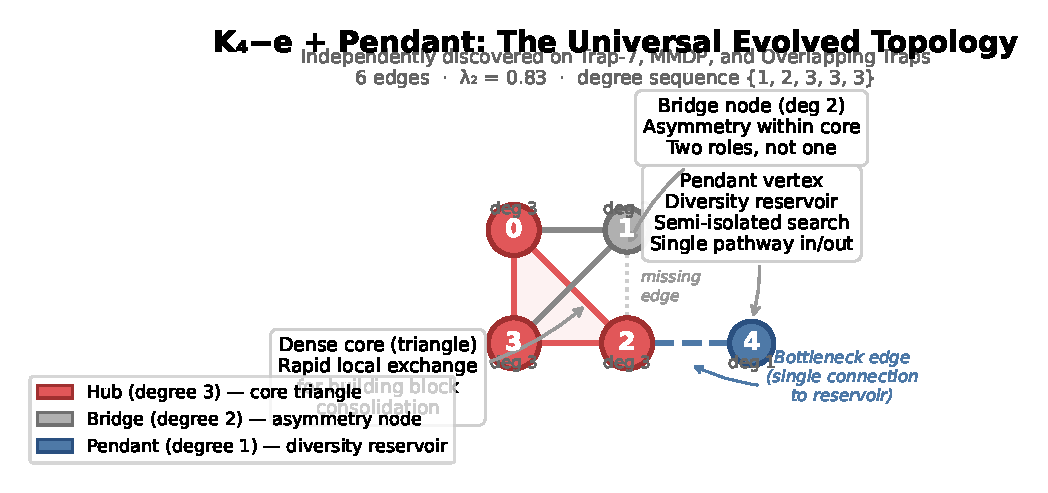
\includegraphics[width=0.85\columnwidth]{../annotated_graph.pdf}
\caption{The universal evolved topology: $K_4 - e$ + pendant.
  Red nodes form the triangle core (rapid local exchange); the blue
  pendant vertex acts as a diversity reservoir connected through a
  single bottleneck edge. The grey bridge node creates asymmetry
  within the core. Independently discovered on 3 of 5 deceptive domains.}
\label{fig:universal}
\end{figure}

\subsection{Functional Interpretation}

Each structural feature has a role in the evolutionary dynamics:

\begin{enumerate}
\item \textbf{Triangle core} (nodes 0, 2, 3): Rapid exchange among
  three islands. A building block discovered on any core island reaches
  the other two within one migration event. This accelerates assembly.

\item \textbf{Pendant vertex} (node 4): Connected to the core through
  a single edge. This island maintains an independent search trajectory,
  acting as a diversity reservoir. Building blocks flow in slowly;
  local optima are less likely to invade.

\item \textbf{Bridge node} (node 1): Degree 2 within a degree-3 core.
  The missing edge (between nodes 1 and 2) creates two distinct roles:
  bridge nodes participate in the core but with reduced coupling,
  providing an intermediate mixing rate.

\item \textbf{Bottleneck edge} (2--4): The single connection to the
  pendant. This creates a bandwidth constraint on migration---building
  blocks must ``earn'' their way into the reservoir by surviving the
  bottleneck.
\end{enumerate}

\subsection{The Two Variants}

The two domains that did not converge to $K_4 - e$ + pendant adapted
the density:

\begin{itemize}
\item \textbf{Trap-5} ($\lambda_2 = 1.38$, 6 edges, no pendant):
  Flat deception with a single attractor. Assembly dominates---slightly
  higher connectivity helps spread building blocks faster.

\item \textbf{HIFF} ($\lambda_2 = 0.52$, 5 edges, pendant):
  Hierarchical deception requiring level-by-level consolidation.
  Sparser connectivity prevents premature mixing of building blocks
  at different hierarchy levels.
\end{itemize}

% ============================================================
% 6. Scaling to n=8
% ============================================================

\section{Scaling}
\label{sec:scaling}

% n=8 results: 28-bit graph genome, 268M search space
% The advantage grows with n

\textbf{TODO:} At $n = 8$ islands (28-bit graph genome, $2^{28}
\approx 268$M possible graphs), the evolved graph beats FC by +0.009
on Trap-5 (vs +0.005 at $n = 5$). The advantage grows with island
count. Evolved graphs at $n = 8$ maintain $\sim$50\% edge density
and heterogeneous degree distribution.

% ============================================================
% 7. Time-Dependent Optimality
% ============================================================

\section{Time-Dependent Optimality}
\label{sec:time}

The evolved graphs were optimized with a 200-generation inner GA.
But is 200 generations the right horizon? We tracked fitness over
500 generations for six topologies on Trap-5 and HIFF (15 seeds each).

\subsection{Topology Rankings Shift Over Time}

\begin{table}[h]
\caption{Best fitness by topology over 2000 generations (Trap-5,
  $n=5$, 15 seeds). Bold = leader at that generation.}
\label{tab:convergence}
\centering
\small
\begin{tabular}{rcccccc}
\toprule
\textbf{Gen} & \textbf{$K_4{-}e{+}$p} & \textbf{FC} & \textbf{Ring} & \textbf{Star} & \textbf{None} & \textbf{HIFF ev.} \\
\midrule
 50  & 0.881 & \textbf{0.895} & 0.883 & 0.871 & 0.847 & 0.872 \\
100  & 0.899 & 0.907 & \textbf{0.908} & 0.893 & 0.856 & 0.899 \\
200  & 0.900 & 0.907 & \textbf{0.913} & 0.911 & 0.853 & 0.911 \\
500  & 0.903 & 0.907 & \textbf{0.924} & 0.913 & 0.853 & 0.921 \\
1000 & 0.903 & 0.915 & \textbf{0.929} & 0.925 & 0.857 & 0.923 \\
2000 & 0.916 & 0.923 & \textbf{0.939} & 0.935 & 0.856 & 0.931 \\
\bottomrule
\end{tabular}
\end{table}

\begin{table}[h]
\caption{Best fitness by topology over 2000 generations (HIFF,
  $n=5$, 15 seeds). Bold = leader at that generation.}
\label{tab:convergence-hiff}
\centering
\small
\begin{tabular}{rcccccc}
\toprule
\textbf{Gen} & \textbf{$K_4{-}e{+}$p} & \textbf{FC} & \textbf{Ring} & \textbf{Star} & \textbf{None} & \textbf{HIFF ev.} \\
\midrule
 50  & \textbf{0.669} & 0.666 & 0.664 & 0.646 & 0.575 & 0.632 \\
100  & \textbf{0.727} & 0.711 & 0.725 & 0.704 & 0.610 & 0.696 \\
200  & 0.743 & 0.741 & \textbf{0.759} & 0.745 & 0.663 & 0.755 \\
500  & 0.785 & 0.760 & 0.797 & 0.761 & 0.706 & \textbf{0.817} \\
1000 & 0.791 & 0.766 & 0.804 & 0.781 & 0.725 & \textbf{0.826} \\
2000 & 0.798 & 0.802 & 0.808 & \textbf{0.844} & 0.763 & 0.829 \\
\bottomrule
\end{tabular}
\end{table}

\textbf{Trap-5:} FC leads at generation~50 (fast assembly), but
\textbf{ring overtakes by generation~100 and never relinquishes the
lead through 2000 generations}. At generation~2000, ring reaches
0.939---still climbing with zero degradation. The $K_4{-}e$ + pendant
graph leads briefly at generation~25 but plateaus by generation~200.

\textbf{HIFF:} The $K_4{-}e$ + pendant leads through generation~100
(fast exploration). The HIFF-evolved graph ($\lambda_2 = 0.52$)
overtakes at generation~300 and leads through generation~1000. But at
generation~1500, \textbf{star overtakes everything}---reaching 0.844
at generation~2000. The hub-spoke structure apparently helps
coordinate hierarchical building block assembly at very long horizons.

Notably, none (isolated islands) shows severe degradation on HIFF:
peak 0.818 then falling to 0.763, a loss of 0.055. Too much isolation
eventually degrades performance---diversity without any exchange
becomes drift.

\subsection{Different Graphs Peak at Different Times}

\subsection{Different Topologies Peak at Different Times}

\begin{table}[h]
\caption{Peak generation and degradation over 2000 generations.}
\label{tab:peaks}
\centering
\begin{tabular}{lrrrr}
\toprule
\textbf{Topology} & \textbf{Trap-5 peak} & \textbf{Trap-5 val} & \textbf{HIFF peak} & \textbf{HIFF val} \\
\midrule
$K_4{-}e$ + pendant  & 1943 & 0.917 & 1944 & 0.810 \\
FC                   & 1823 & 0.924 & 1948 & 0.802 \\
Ring                 & 1999 & 0.939 & 1208 & 0.812 \\
Star                 & 1739 & 0.936 & 1982 & 0.850 \\
None                 &  587 & 0.864 & 1864 & 0.818 \\
HIFF evolved         & 1923 & 0.932 & 1098 & 0.829 \\
\bottomrule
\end{tabular}
\end{table}

Ring is the only topology on Trap-5 that shows \emph{zero degradation}
at 2000 generations---it has not yet peaked. On HIFF, star is still
climbing at generation~1982. The $K_4{-}e$ + pendant graph peaks
earlier: its advantage is speed of convergence, not asymptotic quality.

None (isolated islands) degrades severely on HIFF ($-0.055$ from peak),
confirming that diversity without exchange eventually becomes genetic
drift.

\subsection{Implications for Meta-Evolution}

The inner GA in our outer evolution ran for 200 generations. This means
the outer GA was optimizing for \emph{200-generation fitness}, not
asymptotic fitness. A different inner horizon produces a different
``optimal'' topology:

\begin{itemize}
\item \textbf{Short horizon ($< 100$ gens):} The $K_4{-}e$ + pendant
  graph excels---fast exploration via the triangle core, with the
  pendant preventing premature convergence.
\item \textbf{Medium horizon (100--500 gens):} Ring leads on Trap-5;
  domain-specific evolved graphs lead on HIFF.
\item \textbf{Long horizon ($> 1000$ gens):} Ring dominates Trap-5
  (sustained diversity, zero degradation). Star dominates HIFF
  (hub coordinates hierarchical assembly at scale).
\end{itemize}

Even at 2000 generations, the rankings have not stabilized: ring is
still climbing on Trap-5, star is still climbing on HIFF. The
evaluation horizon is not a nuisance parameter---it is a
\emph{design choice} that determines which topology is optimal.
``Best topology'' is meaningless without specifying ``best at what
generation.''

This result strongly motivates \emph{dynamic topologies}: a schedule
that starts dense (fast assembly via the $K_4{-}e$ + pendant
architecture) and transitions to sparse (sustained search via ring)
would capture the advantages of both regimes.

% ============================================================
% 8. Discussion
% ============================================================

\section{Discussion}
\label{sec:discussion}

\subsection{Connection to the Categorical Framework}

% The laxator's sign depends on landscape structure
% Honest: large ||φ_G|| = bad (diversity erosion)
% Deceptive: large ||φ_G|| = good (assembly) or bad (over-mixing)
% Connects to the coupling sign-flip (Lan vs Ran)

\textbf{TODO:} The laxator $\varphi_G$ from the ACT paper measures
compositional disruption from migration. On honest landscapes this
disruption erodes diversity (harmful). On deceptive landscapes the
same disruption spreads building blocks (helpful) \emph{or} destroys
hierarchical structure (harmful on HIFF). The sign and magnitude of
the laxator's effect depends on landscape structure---formalizing this
is future work.

\subsection{Building Block Theory}

% Goldberg's building block hypothesis: GA works by assembling short,
% high-fitness schemas. Topology controls assembly rate.
% Triangle core = nursery for building blocks
% Pendant = diversity reservoir preventing premature convergence

\textbf{TODO:} Connect to Goldberg's building block hypothesis.
The triangle core accelerates assembly; the pendant prevents
premature convergence. $K_4 - e$ + pendant is the optimal architecture
for balancing these two forces.

\subsection{Limitations}

\begin{itemize}
\item \textbf{Horizon dependence.} The evolved graphs are optimal at
  the 200-generation inner horizon. At 500 generations, ring
  overtakes the evolved graphs on Trap-5. The ``universal topology''
  is universal at a specific time scale.
\item \textbf{Noisy inner fitness.} 5 inner seeds per evaluation
  creates noisy fitness estimates. The evolved graph sometimes loses
  to canonical topologies on 30-seed comparison (MMDP, overlapping
  traps).
\item \textbf{Scale.} The isomorphism result is specific to $n = 5$.
  At $n = 8$ (268M possible graphs), we observe consistent structural
  features but have not confirmed isomorphism across domains.
\item \textbf{Graph genome.} Binary adjacency vectors cannot express
  directed edges, weighted edges, or time-varying topologies---all of
  which might improve performance.
\item \textbf{Honest landscapes.} On OneMax, all topologies perform
  identically (every seed solves the problem). The evolved topology
  is specific to deceptive landscapes; its performance on hard honest
  domains is untested.
\end{itemize}

% ============================================================
% 8. Conclusion
% ============================================================

\section{Conclusion}

Migration topology determines diversity dynamics universally, but the
\emph{value} of that diversity is problem-dependent. On deceptive
landscapes, the fitness ordering inverts, reverses, or shifts to a
Goldilocks zone depending on the deception type.

An outer GA evolving the migration graph discovers $K_4 - e$ + pendant
independently on three of five deceptive domains---a moderately
connected, asymmetric graph with a triangle core and a pendant
diversity reservoir. This convergent evolution across qualitatively
different deceptive landscapes (flat traps, multimodal deception,
inter-block epistasis) is, to our knowledge, the first identification
of a preferred migration architecture for deceptive landscapes.

However, the ``best'' topology is time-dependent. The $K_4 - e$ +
pendant graph excels in early generations (fast exploration), but
sparser topologies overtake it at longer horizons (sustained search).
The evaluation horizon used during meta-evolution is not a nuisance
parameter but a design choice that determines which topology is
optimal. This suggests that the real solution is not a fixed graph
but a \emph{dynamic} topology---one that adapts its connectivity
over the course of evolution, dense early and sparse late.

The central finding is a separation of concerns: $\lambda_2$
determines diversity (a structural invariant), graph \emph{shape}
determines short-horizon fitness (the convergent $K_4 - e$ + pendant),
and the evaluation horizon determines which of these matters more.

% ============================================================
% References
% ============================================================

\bibliographystyle{ACM-Reference-Format}
% \bibliography{references}  % TODO: create references.bib

\begin{thebibliography}{10}

\bibitem{goldberg1987}
D.~E. Goldberg.
\newblock Simple genetic algorithms and the minimal deceptive problem.
\newblock In \emph{Genetic Algorithms and Simulated Annealing}, pp. 74--88, 1987.

\bibitem{goldberg1992}
D.~E. Goldberg, K.~Deb, and J.~Horn.
\newblock Massive multimodality, deception, and genetic algorithms.
\newblock In \emph{PPSN II}, pp. 37--46, 1992.

\bibitem{watson1998}
R.~A. Watson and J.~B. Pollack.
\newblock Hierarchically consistent test problems for genetic algorithms.
\newblock In \emph{PPSN V}, pp. 848--857, 1998.

\bibitem{langer2026}
R.~Langer, C.~Turing, and L.~Vega.
\newblock From games to graphs: Categorical composition of genetic algorithms
  across domains.
\newblock In \emph{ACT 2026} (submitted), 2026.

\bibitem{whitley1999}
D.~Whitley, S.~Rana, and R.~B. Heckendorn.
\newblock The island model genetic algorithm: On separability, population size
  and convergence.
\newblock \emph{Journal of Computing and Information Technology}, 7:33--47, 1999.

\bibitem{skolicki2005}
Z.~Skolicki and K.~De~Jong.
\newblock The influence of migration sizes and intervals on island models.
\newblock In \emph{GECCO 2005}, pp. 1295--1302, 2005.

\bibitem{gavranovic2024}
B.~Gavranovi\'{c} et al.
\newblock Categorical deep learning: An algebraic theory of architectures.
\newblock In \emph{ICML 2024}, 2024.

\end{thebibliography}

\end{document}
